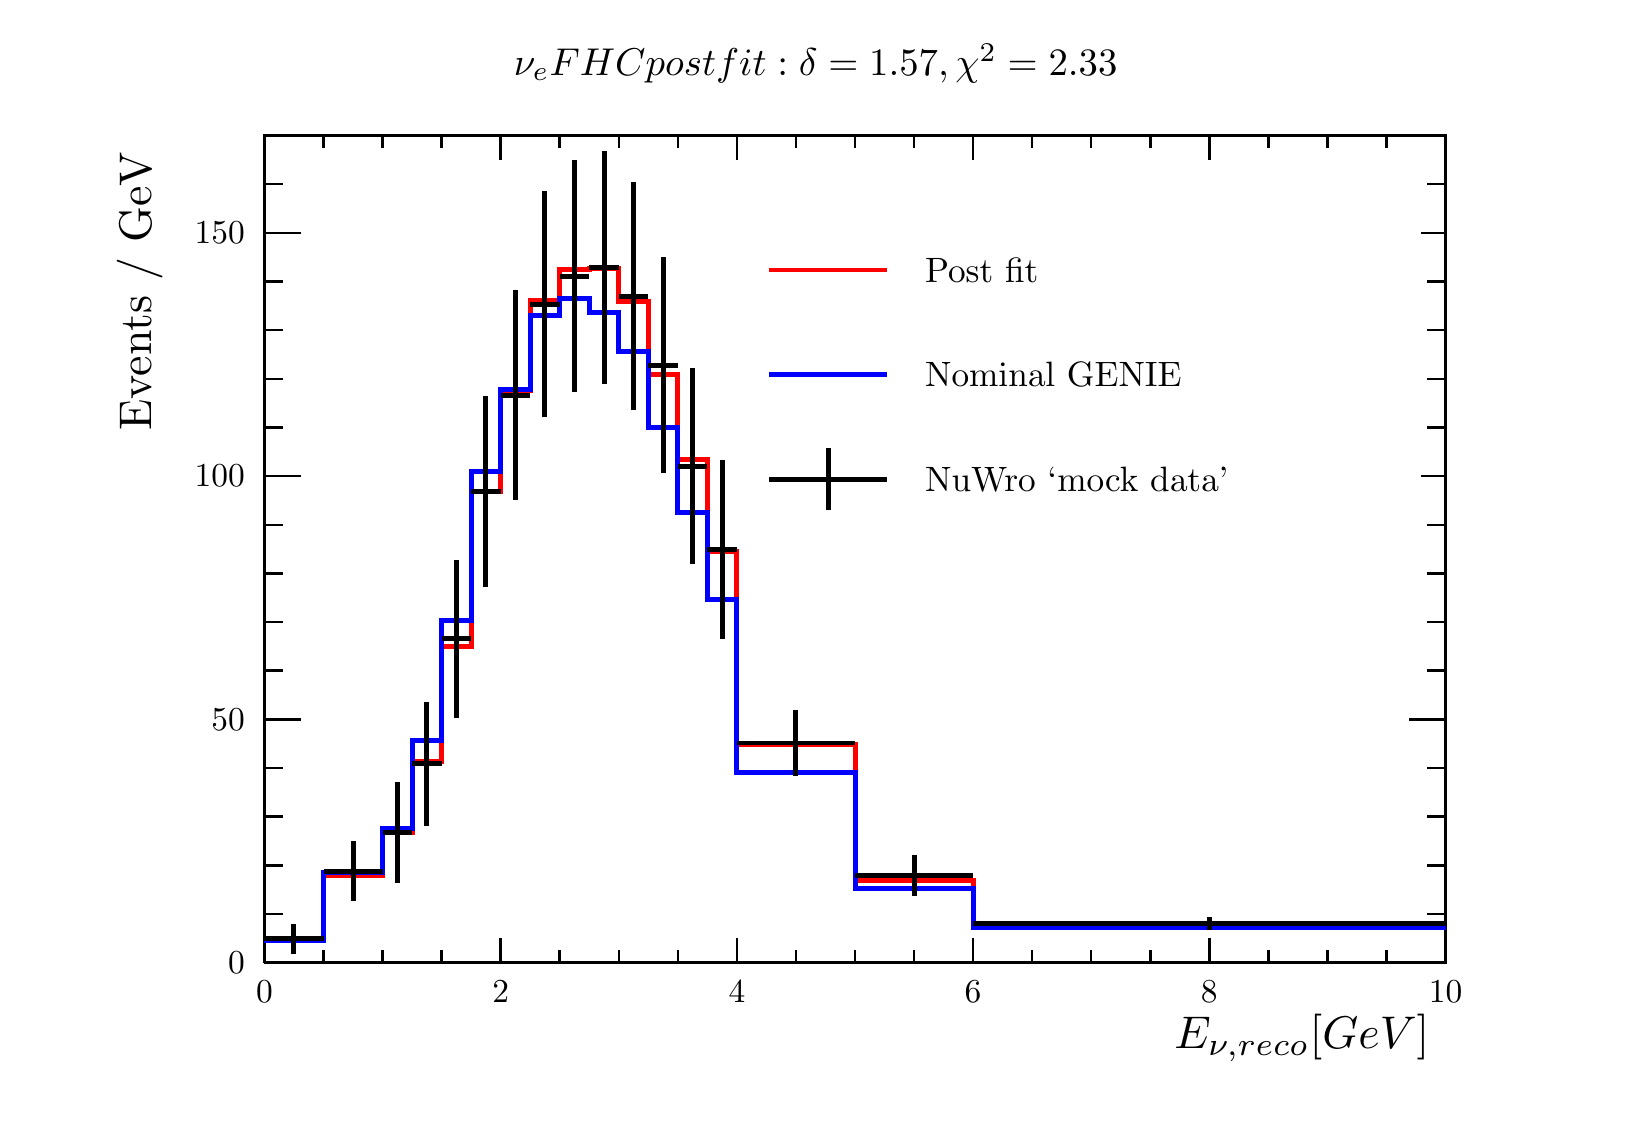
\begin{tikzpicture}
\pgfdeclareplotmark{cross} {
\pgfpathmoveto{\pgfpoint{-0.3\pgfplotmarksize}{\pgfplotmarksize}}
\pgfpathlineto{\pgfpoint{+0.3\pgfplotmarksize}{\pgfplotmarksize}}
\pgfpathlineto{\pgfpoint{+0.3\pgfplotmarksize}{0.3\pgfplotmarksize}}
\pgfpathlineto{\pgfpoint{+1\pgfplotmarksize}{0.3\pgfplotmarksize}}
\pgfpathlineto{\pgfpoint{+1\pgfplotmarksize}{-0.3\pgfplotmarksize}}
\pgfpathlineto{\pgfpoint{+0.3\pgfplotmarksize}{-0.3\pgfplotmarksize}}
\pgfpathlineto{\pgfpoint{+0.3\pgfplotmarksize}{-1.\pgfplotmarksize}}
\pgfpathlineto{\pgfpoint{-0.3\pgfplotmarksize}{-1.\pgfplotmarksize}}
\pgfpathlineto{\pgfpoint{-0.3\pgfplotmarksize}{-0.3\pgfplotmarksize}}
\pgfpathlineto{\pgfpoint{-1.\pgfplotmarksize}{-0.3\pgfplotmarksize}}
\pgfpathlineto{\pgfpoint{-1.\pgfplotmarksize}{0.3\pgfplotmarksize}}
\pgfpathlineto{\pgfpoint{-0.3\pgfplotmarksize}{0.3\pgfplotmarksize}}
\pgfpathclose
\pgfusepathqstroke
}
\pgfdeclareplotmark{cross*} {
\pgfpathmoveto{\pgfpoint{-0.3\pgfplotmarksize}{\pgfplotmarksize}}
\pgfpathlineto{\pgfpoint{+0.3\pgfplotmarksize}{\pgfplotmarksize}}
\pgfpathlineto{\pgfpoint{+0.3\pgfplotmarksize}{0.3\pgfplotmarksize}}
\pgfpathlineto{\pgfpoint{+1\pgfplotmarksize}{0.3\pgfplotmarksize}}
\pgfpathlineto{\pgfpoint{+1\pgfplotmarksize}{-0.3\pgfplotmarksize}}
\pgfpathlineto{\pgfpoint{+0.3\pgfplotmarksize}{-0.3\pgfplotmarksize}}
\pgfpathlineto{\pgfpoint{+0.3\pgfplotmarksize}{-1.\pgfplotmarksize}}
\pgfpathlineto{\pgfpoint{-0.3\pgfplotmarksize}{-1.\pgfplotmarksize}}
\pgfpathlineto{\pgfpoint{-0.3\pgfplotmarksize}{-0.3\pgfplotmarksize}}
\pgfpathlineto{\pgfpoint{-1.\pgfplotmarksize}{-0.3\pgfplotmarksize}}
\pgfpathlineto{\pgfpoint{-1.\pgfplotmarksize}{0.3\pgfplotmarksize}}
\pgfpathlineto{\pgfpoint{-0.3\pgfplotmarksize}{0.3\pgfplotmarksize}}
\pgfpathclose
\pgfusepathqfillstroke
}
\pgfdeclareplotmark{newstar} {
\pgfpathmoveto{\pgfqpoint{0pt}{\pgfplotmarksize}}
\pgfpathlineto{\pgfqpointpolar{44}{0.5\pgfplotmarksize}}
\pgfpathlineto{\pgfqpointpolar{18}{\pgfplotmarksize}}
\pgfpathlineto{\pgfqpointpolar{-20}{0.5\pgfplotmarksize}}
\pgfpathlineto{\pgfqpointpolar{-54}{\pgfplotmarksize}}
\pgfpathlineto{\pgfqpointpolar{-90}{0.5\pgfplotmarksize}}
\pgfpathlineto{\pgfqpointpolar{234}{\pgfplotmarksize}}
\pgfpathlineto{\pgfqpointpolar{198}{0.5\pgfplotmarksize}}
\pgfpathlineto{\pgfqpointpolar{162}{\pgfplotmarksize}}
\pgfpathlineto{\pgfqpointpolar{134}{0.5\pgfplotmarksize}}
\pgfpathclose
\pgfusepathqstroke
}
\pgfdeclareplotmark{newstar*} {
\pgfpathmoveto{\pgfqpoint{0pt}{\pgfplotmarksize}}
\pgfpathlineto{\pgfqpointpolar{44}{0.5\pgfplotmarksize}}
\pgfpathlineto{\pgfqpointpolar{18}{\pgfplotmarksize}}
\pgfpathlineto{\pgfqpointpolar{-20}{0.5\pgfplotmarksize}}
\pgfpathlineto{\pgfqpointpolar{-54}{\pgfplotmarksize}}
\pgfpathlineto{\pgfqpointpolar{-90}{0.5\pgfplotmarksize}}
\pgfpathlineto{\pgfqpointpolar{234}{\pgfplotmarksize}}
\pgfpathlineto{\pgfqpointpolar{198}{0.5\pgfplotmarksize}}
\pgfpathlineto{\pgfqpointpolar{162}{\pgfplotmarksize}}
\pgfpathlineto{\pgfqpointpolar{134}{0.5\pgfplotmarksize}}
\pgfpathclose
\pgfusepathqfillstroke
}
\definecolor{c}{rgb}{1,1,1};
\draw [color=c, fill=c] (0,0) rectangle (20,13.639);
\draw [color=c, fill=c] (3,1.77307) rectangle (18,12.2751);
\definecolor{c}{rgb}{0,0,0};
\draw [c,line width=0.9] (3,1.77307) -- (3,12.2751) -- (18,12.2751) -- (18,1.77307) -- (3,1.77307);
\definecolor{c}{rgb}{1,1,1};
\draw [color=c, fill=c] (3,1.77307) rectangle (18,12.2751);
\definecolor{c}{rgb}{0,0,0};
\draw [c,line width=0.9] (3,1.77307) -- (3,12.2751) -- (18,12.2751) -- (18,1.77307) -- (3,1.77307);
\definecolor{c}{rgb}{1,0,0};
\draw [c,line width=1.8] (3,2.059) -- (3.75,2.059) -- (3.75,2.87639) -- (4.5,2.87639) -- (4.5,3.42495) -- (4.875,3.42495) -- (4.875,4.33215) -- (5.25,4.33215) -- (5.25,5.78427) -- (5.625,5.78427) -- (5.625,7.76137) -- (6,7.76137) -- (6,9.04359) --
 (6.375,9.04359) -- (6.375,10.1806) -- (6.75,10.1806) -- (6.75,10.5725) -- (7.125,10.5725) -- (7.125,10.5838) -- (7.5,10.5838) -- (7.5,10.1744) -- (7.875,10.1744) -- (7.875,9.23699) -- (8.25,9.23699) -- (8.25,8.16016) -- (8.625,8.16016) --
 (8.625,6.99668) -- (9,6.99668) -- (9,4.54455) -- (10.5,4.54455) -- (10.5,2.81665) -- (12,2.81665) -- (12,2.25012) -- (18,2.25012);
\definecolor{c}{rgb}{0,0,0};
\draw [c,line width=0.9] (3,1.77307) -- (18,1.77307);
\draw [c,line width=0.9] (3,2.07994) -- (3,1.77307);
\draw [c,line width=0.9] (3.75,1.9265) -- (3.75,1.77307);
\draw [c,line width=0.9] (4.5,1.9265) -- (4.5,1.77307);
\draw [c,line width=0.9] (5.25,1.9265) -- (5.25,1.77307);
\draw [c,line width=0.9] (6,2.07994) -- (6,1.77307);
\draw [c,line width=0.9] (6.75,1.9265) -- (6.75,1.77307);
\draw [c,line width=0.9] (7.5,1.9265) -- (7.5,1.77307);
\draw [c,line width=0.9] (8.25,1.9265) -- (8.25,1.77307);
\draw [c,line width=0.9] (9,2.07994) -- (9,1.77307);
\draw [c,line width=0.9] (9.75,1.9265) -- (9.75,1.77307);
\draw [c,line width=0.9] (10.5,1.9265) -- (10.5,1.77307);
\draw [c,line width=0.9] (11.25,1.9265) -- (11.25,1.77307);
\draw [c,line width=0.9] (12,2.07994) -- (12,1.77307);
\draw [c,line width=0.9] (12.75,1.9265) -- (12.75,1.77307);
\draw [c,line width=0.9] (13.5,1.9265) -- (13.5,1.77307);
\draw [c,line width=0.9] (14.25,1.9265) -- (14.25,1.77307);
\draw [c,line width=0.9] (15,2.07994) -- (15,1.77307);
\draw [c,line width=0.9] (15.75,1.9265) -- (15.75,1.77307);
\draw [c,line width=0.9] (16.5,1.9265) -- (16.5,1.77307);
\draw [c,line width=0.9] (17.25,1.9265) -- (17.25,1.77307);
\draw [c,line width=0.9] (18,2.07994) -- (18,1.77307);
\draw [anchor=base] (3,1.26842) node[scale=1.20912, color=c, rotate=0]{0};
\draw [anchor=base] (6,1.26842) node[scale=1.20912, color=c, rotate=0]{2};
\draw [anchor=base] (9,1.26842) node[scale=1.20912, color=c, rotate=0]{4};
\draw [anchor=base] (12,1.26842) node[scale=1.20912, color=c, rotate=0]{6};
\draw [anchor=base] (15,1.26842) node[scale=1.20912, color=c, rotate=0]{8};
\draw [anchor=base] (18,1.26842) node[scale=1.20912, color=c, rotate=0]{10};
\draw [anchor= east] (18,0.812882) node[scale=1.65459, color=c, rotate=0]{$E_{\nu, reco} [GeV]$};
\draw [c,line width=0.9] (3,12.2751) -- (18,12.2751);
\draw [c,line width=0.9] (3,11.9682) -- (3,12.2751);
\draw [c,line width=0.9] (3.75,12.1216) -- (3.75,12.2751);
\draw [c,line width=0.9] (4.5,12.1216) -- (4.5,12.2751);
\draw [c,line width=0.9] (5.25,12.1216) -- (5.25,12.2751);
\draw [c,line width=0.9] (6,11.9682) -- (6,12.2751);
\draw [c,line width=0.9] (6.75,12.1216) -- (6.75,12.2751);
\draw [c,line width=0.9] (7.5,12.1216) -- (7.5,12.2751);
\draw [c,line width=0.9] (8.25,12.1216) -- (8.25,12.2751);
\draw [c,line width=0.9] (9,11.9682) -- (9,12.2751);
\draw [c,line width=0.9] (9.75,12.1216) -- (9.75,12.2751);
\draw [c,line width=0.9] (10.5,12.1216) -- (10.5,12.2751);
\draw [c,line width=0.9] (11.25,12.1216) -- (11.25,12.2751);
\draw [c,line width=0.9] (12,11.9682) -- (12,12.2751);
\draw [c,line width=0.9] (12.75,12.1216) -- (12.75,12.2751);
\draw [c,line width=0.9] (13.5,12.1216) -- (13.5,12.2751);
\draw [c,line width=0.9] (14.25,12.1216) -- (14.25,12.2751);
\draw [c,line width=0.9] (15,11.9682) -- (15,12.2751);
\draw [c,line width=0.9] (15.75,12.1216) -- (15.75,12.2751);
\draw [c,line width=0.9] (16.5,12.1216) -- (16.5,12.2751);
\draw [c,line width=0.9] (17.25,12.1216) -- (17.25,12.2751);
\draw [c,line width=0.9] (18,11.9682) -- (18,12.2751);
\draw [c,line width=0.9] (3,1.77307) -- (3,12.2751);
\draw [c,line width=0.9] (3.462,1.77307) -- (3,1.77307);
\draw [c,line width=0.9] (3.231,2.39083) -- (3,2.39083);
\draw [c,line width=0.9] (3.231,3.0086) -- (3,3.0086);
\draw [c,line width=0.9] (3.231,3.62636) -- (3,3.62636);
\draw [c,line width=0.9] (3.231,4.24413) -- (3,4.24413);
\draw [c,line width=0.9] (3.462,4.86189) -- (3,4.86189);
\draw [c,line width=0.9] (3.231,5.47966) -- (3,5.47966);
\draw [c,line width=0.9] (3.231,6.09742) -- (3,6.09742);
\draw [c,line width=0.9] (3.231,6.71519) -- (3,6.71519);
\draw [c,line width=0.9] (3.231,7.33295) -- (3,7.33295);
\draw [c,line width=0.9] (3.462,7.95072) -- (3,7.95072);
\draw [c,line width=0.9] (3.231,8.56848) -- (3,8.56848);
\draw [c,line width=0.9] (3.231,9.18625) -- (3,9.18625);
\draw [c,line width=0.9] (3.231,9.80401) -- (3,9.80401);
\draw [c,line width=0.9] (3.231,10.4218) -- (3,10.4218);
\draw [c,line width=0.9] (3.462,11.0395) -- (3,11.0395);
\draw [c,line width=0.9] (3.462,11.0395) -- (3,11.0395);
\draw [c,line width=0.9] (3.231,11.6573) -- (3,11.6573);
\draw [c,line width=0.9] (3.231,12.2751) -- (3,12.2751);
\draw [anchor= east] (2.9,1.77307) node[scale=1.20912, color=c, rotate=0]{0};
\draw [anchor= east] (2.9,4.86189) node[scale=1.20912, color=c, rotate=0]{50};
\draw [anchor= east] (2.9,7.95072) node[scale=1.20912, color=c, rotate=0]{100};
\draw [anchor= east] (2.9,11.0395) node[scale=1.20912, color=c, rotate=0]{150};
\draw [anchor= east] (1.416,12.2751) node[scale=1.65459, color=c, rotate=90]{Events / GeV};
\draw [c,line width=0.9] (18,1.77307) -- (18,12.2751);
\draw [c,line width=0.9] (17.538,1.77307) -- (18,1.77307);
\draw [c,line width=0.9] (17.769,2.39083) -- (18,2.39083);
\draw [c,line width=0.9] (17.769,3.0086) -- (18,3.0086);
\draw [c,line width=0.9] (17.769,3.62636) -- (18,3.62636);
\draw [c,line width=0.9] (17.769,4.24413) -- (18,4.24413);
\draw [c,line width=0.9] (17.538,4.86189) -- (18,4.86189);
\draw [c,line width=0.9] (17.769,5.47966) -- (18,5.47966);
\draw [c,line width=0.9] (17.769,6.09742) -- (18,6.09742);
\draw [c,line width=0.9] (17.769,6.71519) -- (18,6.71519);
\draw [c,line width=0.9] (17.769,7.33295) -- (18,7.33295);
\draw [c,line width=0.9] (17.538,7.95072) -- (18,7.95072);
\draw [c,line width=0.9] (17.769,8.56848) -- (18,8.56848);
\draw [c,line width=0.9] (17.769,9.18625) -- (18,9.18625);
\draw [c,line width=0.9] (17.769,9.80401) -- (18,9.80401);
\draw [c,line width=0.9] (17.769,10.4218) -- (18,10.4218);
\draw [c,line width=0.9] (17.538,11.0395) -- (18,11.0395);
\draw [c,line width=0.9] (17.538,11.0395) -- (18,11.0395);
\draw [c,line width=0.9] (17.769,11.6573) -- (18,11.6573);
\draw [c,line width=0.9] (17.769,12.2751) -- (18,12.2751);
\definecolor{c}{rgb}{0,0,1};
\draw [c,line width=1.8] (3,2.05641) -- (3.75,2.05641) -- (3.75,2.91454) -- (4.5,2.91454) -- (4.5,3.47351) -- (4.875,3.47351) -- (4.875,4.59637) -- (5.25,4.59637) -- (5.25,6.11824) -- (5.625,6.11824) -- (5.625,8.00335) -- (6,8.00335) -- (6,9.04493)
 -- (6.375,9.04493) -- (6.375,9.99639) -- (6.75,9.99639) -- (6.75,10.2112) -- (7.125,10.2112) -- (7.125,10.0325) -- (7.5,10.0325) -- (7.5,9.53636) -- (7.875,9.53636) -- (7.875,8.57037) -- (8.25,8.57037) -- (8.25,7.48969) -- (8.625,7.48969) --
 (8.625,6.38331) -- (9,6.38331) -- (9,4.18909) -- (10.5,4.18909) -- (10.5,2.71623) -- (12,2.71623) -- (12,2.21727) -- (18,2.21727);
\definecolor{c}{rgb}{0,0,0};
\draw [c,line width=1.8] (3.375,1.88152) -- (3.375,2.07451);
\draw [c,line width=1.8] (3.375,2.07451) -- (3.375,2.26749);
\draw [c,line width=1.8] (3,2.07451) -- (3.375,2.07451);
\draw [c,line width=1.8] (3.375,2.07451) -- (3.75,2.07451);
\foreach \P in {(3.375,2.07451)}{\draw[mark options={color=c,fill=c},mark size=2.402402pt, line width=0.000000pt, mark=*,mark size=1pt] plot coordinates {\P};}
\draw [c,line width=1.8] (4.125,2.55512) -- (4.125,2.93382);
\draw [c,line width=1.8] (4.125,2.93382) -- (4.125,3.31252);
\draw [c,line width=1.8] (3.75,2.93382) -- (4.125,2.93382);
\draw [c,line width=1.8] (4.125,2.93382) -- (4.5,2.93382);
\foreach \P in {(4.125,2.93382)}{\draw[mark options={color=c,fill=c},mark size=2.402402pt, line width=0.000000pt, mark=*,mark size=1pt] plot coordinates {\P};}
\draw [c,line width=1.8] (4.6875,2.78708) -- (4.6875,3.42622);
\draw [c,line width=1.8] (4.6875,3.42622) -- (4.6875,4.06536);
\draw [c,line width=1.8] (4.5,3.42622) -- (4.6875,3.42622);
\draw [c,line width=1.8] (4.6875,3.42622) -- (4.875,3.42622);
\foreach \P in {(4.6875,3.42622)}{\draw[mark options={color=c,fill=c},mark size=2.402402pt, line width=0.000000pt, mark=*,mark size=1pt] plot coordinates {\P};}
\draw [c,line width=1.8] (5.0625,3.50808) -- (5.0625,4.29796);
\draw [c,line width=1.8] (5.0625,4.29796) -- (5.0625,5.08784);
\draw [c,line width=1.8] (4.875,4.29796) -- (5.0625,4.29796);
\draw [c,line width=1.8] (5.0625,4.29796) -- (5.25,4.29796);
\foreach \P in {(5.0625,4.29796)}{\draw[mark options={color=c,fill=c},mark size=2.402402pt, line width=0.000000pt, mark=*,mark size=1pt] plot coordinates {\P};}
\draw [c,line width=1.8] (5.4375,4.87477) -- (5.4375,5.88247);
\draw [c,line width=1.8] (5.4375,5.88247) -- (5.4375,6.89017);
\draw [c,line width=1.8] (5.25,5.88247) -- (5.4375,5.88247);
\draw [c,line width=1.8] (5.4375,5.88247) -- (5.625,5.88247);
\foreach \P in {(5.4375,5.88247)}{\draw[mark options={color=c,fill=c},mark size=2.402402pt, line width=0.000000pt, mark=*,mark size=1pt] plot coordinates {\P};}
\draw [c,line width=1.8] (5.8125,6.5417) -- (5.8125,7.75779);
\draw [c,line width=1.8] (5.8125,7.75779) -- (5.8125,8.97387);
\draw [c,line width=1.8] (5.625,7.75779) -- (5.8125,7.75779);
\draw [c,line width=1.8] (5.8125,7.75779) -- (6,7.75779);
\foreach \P in {(5.8125,7.75779)}{\draw[mark options={color=c,fill=c},mark size=2.402402pt, line width=0.000000pt, mark=*,mark size=1pt] plot coordinates {\P};}
\draw [c,line width=1.8] (6.1875,7.6446) -- (6.1875,8.97901);
\draw [c,line width=1.8] (6.1875,8.97901) -- (6.1875,10.3134);
\draw [c,line width=1.8] (6,8.97901) -- (6.1875,8.97901);
\draw [c,line width=1.8] (6.1875,8.97901) -- (6.375,8.97901);
\foreach \P in {(6.1875,8.97901)}{\draw[mark options={color=c,fill=c},mark size=2.402402pt, line width=0.000000pt, mark=*,mark size=1pt] plot coordinates {\P};}
\draw [c,line width=1.8] (6.5625,8.69782) -- (6.5625,10.1353);
\draw [c,line width=1.8] (6.5625,10.1353) -- (6.5625,11.5728);
\draw [c,line width=1.8] (6.375,10.1353) -- (6.5625,10.1353);
\draw [c,line width=1.8] (6.5625,10.1353) -- (6.75,10.1353);
\foreach \P in {(6.5625,10.1353)}{\draw[mark options={color=c,fill=c},mark size=2.402402pt, line width=0.000000pt, mark=*,mark size=1pt] plot coordinates {\P};}
\draw [c,line width=1.8] (6.9375,9.02356) -- (6.9375,10.4913);
\draw [c,line width=1.8] (6.9375,10.4913) -- (6.9375,11.9591);
\draw [c,line width=1.8] (6.75,10.4913) -- (6.9375,10.4913);
\draw [c,line width=1.8] (6.9375,10.4913) -- (7.125,10.4913);
\foreach \P in {(6.9375,10.4913)}{\draw[mark options={color=c,fill=c},mark size=2.402402pt, line width=0.000000pt, mark=*,mark size=1pt] plot coordinates {\P};}
\draw [c,line width=1.8] (7.3125,9.12259) -- (7.3125,10.5994);
\draw [c,line width=1.8] (7.3125,10.5994) -- (7.3125,12.0763);
\draw [c,line width=1.8] (7.125,10.5994) -- (7.3125,10.5994);
\draw [c,line width=1.8] (7.3125,10.5994) -- (7.5,10.5994);
\foreach \P in {(7.3125,10.5994)}{\draw[mark options={color=c,fill=c},mark size=2.402402pt, line width=0.000000pt, mark=*,mark size=1pt] plot coordinates {\P};}
\draw [c,line width=1.8] (7.6875,8.78946) -- (7.6875,10.2355);
\draw [c,line width=1.8] (7.6875,10.2355) -- (7.6875,11.6816);
\draw [c,line width=1.8] (7.5,10.2355) -- (7.6875,10.2355);
\draw [c,line width=1.8] (7.6875,10.2355) -- (7.875,10.2355);
\foreach \P in {(7.6875,10.2355)}{\draw[mark options={color=c,fill=c},mark size=2.402402pt, line width=0.000000pt, mark=*,mark size=1pt] plot coordinates {\P};}
\draw [c,line width=1.8] (8.0625,7.99097) -- (8.0625,9.36021);
\draw [c,line width=1.8] (8.0625,9.36021) -- (8.0625,10.7295);
\draw [c,line width=1.8] (7.875,9.36021) -- (8.0625,9.36021);
\draw [c,line width=1.8] (8.0625,9.36021) -- (8.25,9.36021);
\foreach \P in {(8.0625,9.36021)}{\draw[mark options={color=c,fill=c},mark size=2.402402pt, line width=0.000000pt, mark=*,mark size=1pt] plot coordinates {\P};}
\draw [c,line width=1.8] (8.4375,6.8301) -- (8.4375,8.07833);
\draw [c,line width=1.8] (8.4375,8.07833) -- (8.4375,9.32656);
\draw [c,line width=1.8] (8.25,8.07833) -- (8.4375,8.07833);
\draw [c,line width=1.8] (8.4375,8.07833) -- (8.625,8.07833);
\foreach \P in {(8.4375,8.07833)}{\draw[mark options={color=c,fill=c},mark size=2.402402pt, line width=0.000000pt, mark=*,mark size=1pt] plot coordinates {\P};}
\draw [c,line width=1.8] (8.8125,5.88043) -- (8.8125,7.01898);
\draw [c,line width=1.8] (8.8125,7.01898) -- (8.8125,8.15753);
\draw [c,line width=1.8] (8.625,7.01898) -- (8.8125,7.01898);
\draw [c,line width=1.8] (8.8125,7.01898) -- (9,7.01898);
\foreach \P in {(8.8125,7.01898)}{\draw[mark options={color=c,fill=c},mark size=2.402402pt, line width=0.000000pt, mark=*,mark size=1pt] plot coordinates {\P};}
\draw [c,line width=1.8] (9.75,4.14636) -- (9.75,4.56139);
\draw [c,line width=1.8] (9.75,4.56139) -- (9.75,4.97643);
\draw [c,line width=1.8] (9,4.56139) -- (9.75,4.56139);
\draw [c,line width=1.8] (9.75,4.56139) -- (10.5,4.56139);
\foreach \P in {(9.75,4.56139)}{\draw[mark options={color=c,fill=c},mark size=2.402402pt, line width=0.000000pt, mark=*,mark size=1pt] plot coordinates {\P};}
\draw [c,line width=1.8] (11.25,2.62032) -- (11.25,2.88207);
\draw [c,line width=1.8] (11.25,2.88207) -- (11.25,3.14381);
\draw [c,line width=1.8] (10.5,2.88207) -- (11.25,2.88207);
\draw [c,line width=1.8] (11.25,2.88207) -- (12,2.88207);
\foreach \P in {(11.25,2.88207)}{\draw[mark options={color=c,fill=c},mark size=2.402402pt, line width=0.000000pt, mark=*,mark size=1pt] plot coordinates {\P};}
\draw [c,line width=1.8] (15,2.18065) -- (15,2.26808);
\draw [c,line width=1.8] (15,2.26808) -- (15,2.35552);
\draw [c,line width=1.8] (12,2.26808) -- (15,2.26808);
\draw [c,line width=1.8] (15,2.26808) -- (18,2.26808);
\foreach \P in {(15,2.26808)}{\draw[mark options={color=c,fill=c},mark size=2.402402pt, line width=0.000000pt, mark=*,mark size=1pt] plot coordinates {\P};}
\definecolor{c}{rgb}{1,1,1};
\draw [color=c, fill=c] (2,12.8206) rectangle (18,13.5708);
\definecolor{c}{rgb}{0,0,0};
\draw (10,13.1957) node[scale=1.40004, color=c, rotate=0]{$\nu_{e} FHC postfit: \delta = 1.57, \chi^{2} = 2.33$};
\definecolor{c}{rgb}{1,1,1};
\draw [color=c, fill=c] (9.08309,7.24928) rectangle (17.6791,11.2321);
\definecolor{c}{rgb}{0,0,0};
\draw [anchor= west] (11.2321,10.5683) node[scale=1.27276, color=c, rotate=0]{Post fit};
\definecolor{c}{rgb}{1,0,0};
\draw [c,line width=1.8] (9.40544,10.5683) -- (10.9097,10.5683);
\definecolor{c}{rgb}{0,0,0};
\draw [anchor= west] (11.2321,9.24069) node[scale=1.27276, color=c, rotate=0]{Nominal GENIE};
\definecolor{c}{rgb}{0,0,1};
\draw [c,line width=1.8] (9.40544,9.24069) -- (10.9097,9.24069);
\definecolor{c}{rgb}{0,0,0};
\draw [anchor= west] (11.2321,7.91308) node[scale=1.27276, color=c, rotate=0]{NuWro `mock data'};
\draw [c,line width=1.8] (9.40544,7.91308) -- (10.9097,7.91308);
\draw [c,line width=1.8] (10.1576,7.5148) -- (10.1576,8.31137);
\end{tikzpicture}
